\subsection{Tracking}

It is neccessary to track the foreground objects to measure their speed and position. Each object's location in an image is determined by a centroid calcuated from their respective bounding boxes. A list of centroids is maintained and new centroids are calculated for each new image, if a new centroid's position is sufficiently close to an old centroid it is assumed to be the new position of that old centroid. Furthermore, if a new centroid is not found for an old centroid in a new image frame then that old centroid has a limited amount of frames before it is dismissed which can occur if it's object leaves the frame is occluded by another object or otherwise is no longer being recognised as a foreground object by the detection process. These latter situations can arise if the view of a vehicle is blocked by another, if the vehicle is shadowed by another making its pixel values darker and more similar to the background or if the vehicle is stationary the GMM will begin to update itself perceiving these unchanging pixels as background. Generally these scenarios do not cause a problem if the system is calibrated correctly and the camera angle is favorable and pertaining to the situation of vehicle being stationary once they begin to move they will be recognised as vehicles once more. In Figure \ref{fig:centroids} the centroids are visualized on the objects along with a unique identifier which is used to mark ownership of a foreground object. The implementation of the tracking design was based heavily on the work of Adrian Rosebrock as outlined in his tutorial series on PyImageSearch \cite{adrian_rosebrock_simple_object_tracking}. Notice in Figure \ref{fig:centroids} centroids 25 and 24 belong to no object, this is because they have not yet timed out, meaning their object hasn't been missing from frame long enough for them to be dismissed, this is also the case for centroid 16. Centroids 1 and 9 belong to a cluster of vehicles that have become distant (see Figure \ref{fig:original_frame}), this occurs because as the vehicles travel further away the distance between them in pixels becomes less and so the morphological process presses them together. This is not an issue if the counting and measuring system is calibrated to focus on areas where vehicles are easily separable (section \ref{subsection:count_measure} and section \ref{subsection:calibration}).   


\begin{figure}[H]
    \centering
    \centering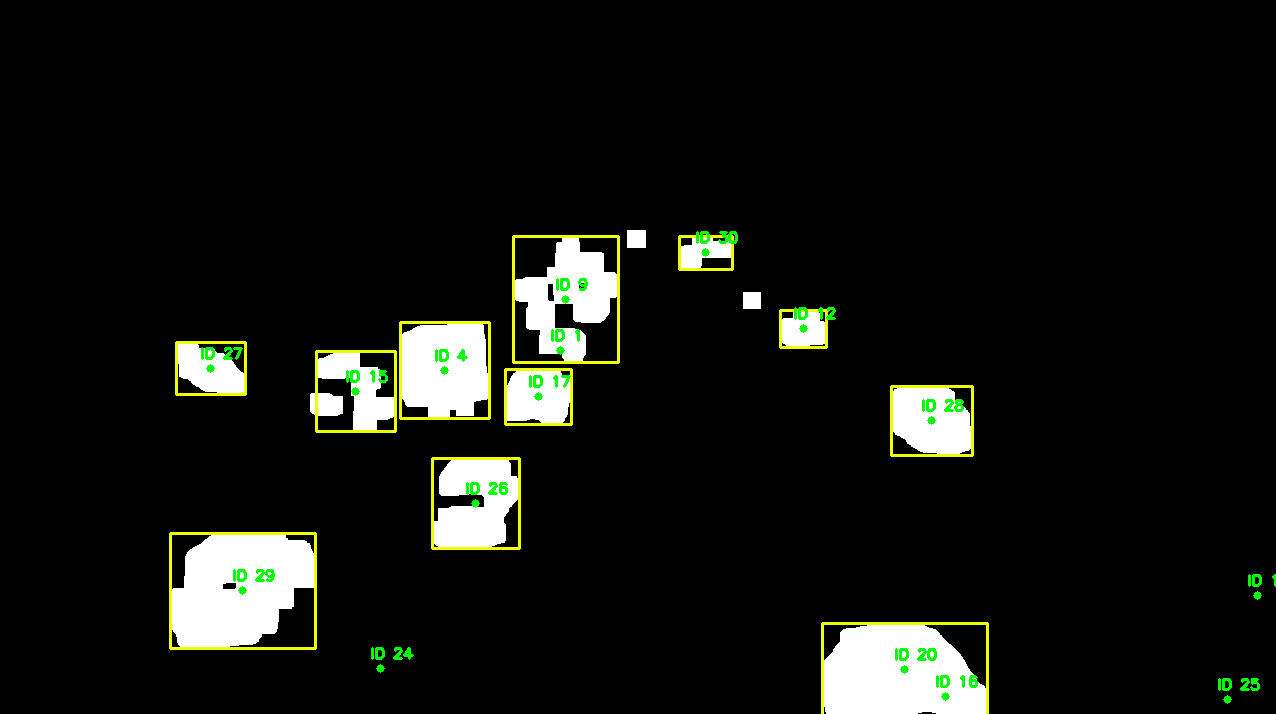
\includegraphics[width = 0.8\textwidth]{design/detection/tracking/mask_centroids}
    \caption{Centroids plotted over foreground objects.}
    \label{fig:centroids}
  \end{figure}
  
